\documentclass[aspectratio=169,11pt]{beamer}
\usepackage[utf8]{inputenc}
\usepackage[T1]{fontenc}
\usepackage{helvet}
\usepackage{tikz}
\usepackage{booktabs}
\usepackage{array}
\usetikzlibrary{arrows.meta,positioning,shapes.misc,calc}

% ---- palette: matches the app ----
\definecolor{ivory}{HTML}{FAF9F5}
\definecolor{ink}{HTML}{1F1E1B}
\definecolor{muted}{HTML}{6E6B63}
\definecolor{clay}{HTML}{C96442}
\definecolor{clayd}{HTML}{B25638}
\definecolor{line}{HTML}{E4E1D7}
\definecolor{card}{HTML}{FFFFFF}
\definecolor{okg}{HTML}{0B6B3A}

\setbeamercolor{background canvas}{bg=ivory}
\setbeamercolor{normal text}{fg=ink}
\setbeamercolor{structure}{fg=clay}
\setbeamercolor{frametitle}{fg=ink,bg=ivory}
\setbeamercolor{title}{fg=ink}
\setbeamerfont{frametitle}{family=\rmfamily,size=\Large,series=\mdseries}
\setbeamerfont{title}{family=\rmfamily,size=\Huge,series=\mdseries}
\setbeamertemplate{navigation symbols}{}
\setbeamertemplate{itemize item}{\textcolor{clay}{\rule[0.4ex]{0.7ex}{0.7ex}}}
\setbeamertemplate{itemize subitem}{\textcolor{muted}{--}}
\setbeamertemplate{frametitle}{\vspace{0.8em}\usebeamerfont{frametitle}\insertframetitle\par\vspace{0.15em}{\color{line}\hrule height 1pt}\vspace{0.2em}}
\setbeamertemplate{footline}{\hfill{\color{muted}\scriptsize\insertframenumber\hspace{2em}}\vspace{0.6em}}

\newcommand{\kicker}[1]{{\color{clay}\scriptsize\bfseries\MakeUppercase{#1}}\\[0.3em]}
\newcommand{\mutedtext}[1]{{\color{muted}#1}}

\title{Gemma Without Borders}
\author{}
\date{}

\begin{document}

% ---------------------------------------------------------------- 1 TITLE
\begin{frame}
  \begin{center}
    \vspace{1.2em}
    \kicker{GDG Windsor · Build with AI · Edge / On-Device Track}
    {\rmfamily\fontsize{34}{38}\selectfont Gemma Without Borders\par}
    \vspace{0.6em}
    {\large An autonomous study agent for the Grade 9 EQAO math assessment.\par}
    \vspace{0.4em}
    \mutedtext{Runs entirely on the student's device. A child's mistakes never leave their machine.}\par
    \vspace{1.6em}
    {\small Gokulakrishnan \,·\, Padmanabha \,·\, Taha \,·\, Naimah \,·\, Amarah}
  \end{center}
\end{frame}

% ---------------------------------------------------------------- 2 PROBLEM
\begin{frame}{The problem: wrong answers are symptoms, not causes}
  \begin{columns}[T]
    \begin{column}{0.55\textwidth}
      \begin{itemize}\setlength\itemsep{0.7em}
        \item Every Ontario Grade 9 student writes the EQAO math assessment. Many arrive with \textbf{specific, well-documented tricks} --- wrong ideas that feel right, not general weakness.
        \item A student who answers $\tfrac{2}{3}+\tfrac{1}{4}=\tfrac{3}{7}$ doesn't need more practice. They need someone to notice they \textbf{add tops and bottoms straight across} --- and fix exactly that.
        \item Teachers can't do this per-student, per-trick. Generic review apps don't even try.
      \end{itemize}
    \end{column}
    \begin{column}{0.41\textwidth}
      \begin{tikzpicture}[scale=0.9]
        \node[draw=line, fill=card, rounded corners=2pt, inner sep=8pt, text width=5.2cm, align=left] at (0,0) {
          {\small Calculate $\tfrac{2}{3}+\tfrac{1}{4}$}\\[3pt]
          {\small A) $\tfrac{11}{12}$ \hfill {\color{okg}\scriptsize correct}}\\[2pt]
          {\small \textbf{B) $\tfrac{3}{7}$} \hfill {\color{clay}\scriptsize adds straight across}}\\[2pt]
          {\small C) $\tfrac{3}{12}$ \hfill {\color{muted}\scriptsize didn't rescale tops}}\\[2pt]
          {\small D) $\tfrac{11}{7}$ \hfill {\color{muted}\scriptsize mixed method}}\\[4pt]
          {\scriptsize\color{muted} Every wrong option is the exact result of a \emph{known} trick --- so the wrong answer itself is the diagnosis.}
        };
      \end{tikzpicture}
    \end{column}
  \end{columns}
\end{frame}

% ---------------------------------------------------------------- 3 WHAT WE BUILT
\begin{frame}{What we built}
  \begin{center}
  \resizebox{\textwidth}{!}{%
  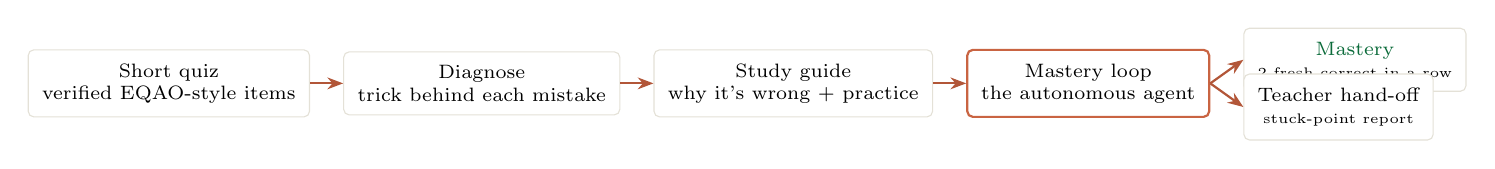
\begin{tikzpicture}[
      node distance=0.45cm and 0.42cm,
      box/.style={draw=line, fill=card, rounded corners=2pt, inner sep=5pt, align=center, font=\scriptsize},
      accent/.style={draw=clay, thick, fill=card, rounded corners=2pt, inner sep=5pt, align=center, font=\scriptsize},
      arr/.style={-{Stealth[length=2mm]}, thick, color=clayd}]
    \node[box] (quiz) {Short quiz\\ \scriptsize verified EQAO-style items};
    \node[box, right=of quiz] (diag) {Diagnose\\ \scriptsize trick behind each mistake};
    \node[box, right=of diag] (guide) {Study guide\\ \scriptsize why it's wrong + practice};
    \node[accent, right=of guide] (loop) {Mastery loop\\ \scriptsize the autonomous agent};
    \node[box, above right=0.3cm and 0.42cm of loop.east, anchor=west] (win) {\color{okg}Mastery\\ \tiny 2 fresh correct in a row};
    \node[box, below right=0.3cm and 0.42cm of loop.east, anchor=west] (esc) {Teacher hand-off\\ \tiny stuck-point report};
    \draw[arr] (quiz) -- (diag);
    \draw[arr] (diag) -- (guide);
    \draw[arr] (guide) -- (loop);
    \draw[arr] (loop.east) -- (win.west);
    \draw[arr] (loop.east) -- (esc.west);
  \end{tikzpicture}}
  \end{center}
  \vspace{0.4em}
  \begin{itemize}\setlength\itemsep{0.4em}
    \item Student takes a 5-question quiz. On submit, the agent reads \textbf{all} the mistakes, finds the pattern, and picks the \textbf{priority trick to untangle}.
    \item Then it \textbf{pursues a goal}: keep teaching --- with different strategies --- until the student \emph{demonstrates} understanding, or a human should take over.
  \end{itemize}
\end{frame}

% ---------------------------------------------------------------- 4 AGENT LOOP
\begin{frame}{An agent, not a chatbot}
  \begin{columns}[T]
    \begin{column}{0.56\textwidth}
      \begin{center}
      \resizebox{\columnwidth}{!}{%
      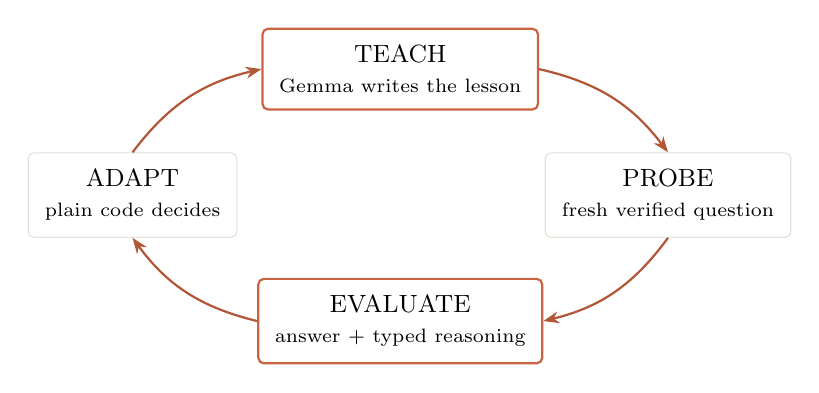
\begin{tikzpicture}[
          box/.style={draw=line, fill=card, rounded corners=2pt, inner sep=6pt, align=center, font=\small, minimum width=2.6cm},
          gbox/.style={draw=clay, thick, fill=card, rounded corners=2pt, inner sep=6pt, align=center, font=\small, minimum width=2.6cm},
          arr/.style={-{Stealth[length=2mm]}, thick, color=clayd}]
        \node[gbox] (teach) at (0,2.4) {TEACH\\ \scriptsize Gemma writes the lesson};
        \node[box] (probe) at (3.4,0.8) {PROBE\\ \scriptsize fresh verified question};
        \node[gbox] (eval) at (0,-0.8) {EVALUATE\\ \scriptsize answer + typed reasoning};
        \node[box] (adapt) at (-3.4,0.8) {ADAPT\\ \scriptsize plain code decides};
        \draw[arr] (teach.east) to[bend left=20] (probe.north);
        \draw[arr] (probe.south) to[bend left=20] (eval.east);
        \draw[arr] (eval.west) to[bend left=20] (adapt.south);
        \draw[arr] (adapt.north) to[bend left=20] (teach.west);
      \end{tikzpicture}}
      \end{center}
    \end{column}
    \begin{column}{0.42\textwidth}
      \textbf{A chatbot responds once.}\\
      \textbf{An agent pursues a goal:}\par
      \vspace{0.3em}
      \mutedtext{\small ``Two consecutive fresh questions answered correctly, with reasoning that shows the trick is gone.''}\par
      \vspace{0.8em}
      \textbf{It cannot run away:}
      \begin{itemize}
        \item {\small 4-attempt cap}
        \item {\small 12-model-call budget}
        \item {\small strategy exhaustion $\rightarrow$ clean teacher hand-off}
      \end{itemize}
      \vspace{0.3em}
      {\scriptsize\color{muted}Orange boxes = Gemma. Every session provably terminates.}
    \end{column}
  \end{columns}
\end{frame}

% ---------------------------------------------------------------- 5 STRATEGY LADDER
\begin{frame}{When a lesson fails, the agent changes how it teaches}
  \begin{center}
  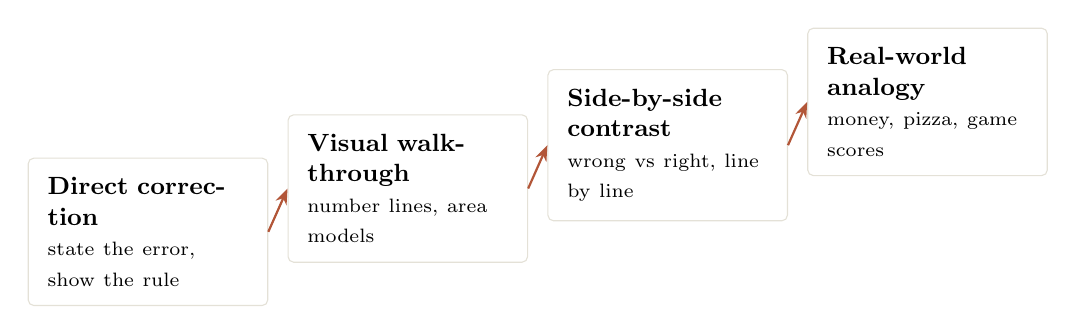
\begin{tikzpicture}[
      rung/.style={draw=line, fill=card, rounded corners=2pt, inner sep=7pt, align=left, text width=2.55cm, font=\small},
      arr/.style={-{Stealth[length=2mm]}, thick, color=clayd}]
    \node[rung] (s0) at (0,0) {\textbf{Direct correction}\\ \scriptsize state the error, show the rule};
    \node[rung] (s1) at (3.3,0.55) {\textbf{Visual walkthrough}\\ \scriptsize number lines, area models};
    \node[rung] (s2) at (6.6,1.1) {\textbf{Side-by-side contrast}\\ \scriptsize wrong vs right, line by line};
    \node[rung] (s3) at (9.9,1.65) {\textbf{Real-world analogy}\\ \scriptsize money, pizza, game scores};
    \draw[arr] (s0.east) -- (s1.west);
    \draw[arr] (s1.east) -- (s2.west);
    \draw[arr] (s2.east) -- (s3.west);
  \end{tikzpicture}
  \end{center}
  \vspace{0.5em}
  \begin{itemize}\setlength\itemsep{0.5em}
    \item Adaptation is a \textbf{fixed ladder} --- every retry is a provably different pedagogy, never an open-ended improvisation.
    \item \textbf{Gemma chooses which rung comes next}, by reading the student's own typed reasoning --- and tells the student why: \mutedtext{\small``Trying a visual walkthrough --- you said you can't see why the denominators matter.''}
    \item Right answer but shaky reasoning? \textbf{Doesn't count toward mastery.} Gemma grades the explanation, not just the bubble.
  \end{itemize}
\end{frame}

% ---------------------------------------------------------------- 6 GEMMA INTEGRATION
\begin{frame}{Where Gemma does the thinking \hfill {\normalsize\color{muted}rubric: Gemma Integration, 30\%}}
  \begin{center}
  \renewcommand{\arraystretch}{1.25}
  {\footnotesize
  \begin{tabular}{@{}p{3.2cm}p{4.4cm}p{5.2cm}@{}}
    \toprule
    \textbf{Gemma's job} & \textbf{Capability shown} & \textbf{Guardrail} \\
    \midrule
    Write the lesson \& explanation & generation, pedagogy & grounded in the verified solution --- may not invent numbers \\
    Grade typed reasoning & reasoning, structured output & closed labels; fail-open; never punishes the student \\
    Choose the next strategy & decision-making & restricted to the remaining ladder; deterministic fallback \\
    Author new questions & structured output (JSON) & must pass its own blind re-solve, else discarded \\
    \bottomrule
  \end{tabular}}
  \end{center}
  \vspace{0.3em}
  \begin{itemize}\setlength\itemsep{0.25em}
    \item {\small Remove Gemma and there is no tutor. \textbf{But the math truth never depends on it.}}
    \item {\small One auditable door (\texttt{gemma\_client.py}); model size is a dial: \texttt{GEMMA\_MODEL=gemma3:12b}.}
  \end{itemize}
\end{frame}

% ---------------------------------------------------------------- 7 VERIFIED BANK
\begin{frame}{The data Gemma stands on \hfill {\normalsize\color{muted}rubric: Functionality, 20\%}}
  \begin{columns}[T]
    \begin{column}{0.5\textwidth}
      \textbf{A verified diagnostic bank:}
      \begin{itemize}\setlength\itemsep{0.45em}
        \item {\small 36 original EQAO-style questions across all 5 strands of the Ontario MTH1W curriculum}
        \item {\small a taxonomy of 48 tricks, each with the flawed thinking spelled out}
        \item {\small every wrong option tagged with the trick that produces it}
        \item {\small independently re-solved and adversarially checked; 10 tags corrected in review}
      \end{itemize}
    \end{column}
    \begin{column}{0.47\textwidth}
      \textbf{So the agent can be trusted:}
      \begin{itemize}\setlength\itemsep{0.45em}
        \item {\small \textbf{Diagnosis} = table lookup on the tags. No model call, no hallucination, 100\% reproducible.}
        \item {\small \textbf{Probes} are served bank-first --- a generated question is a last resort, and must audit itself.}
        \item {\small \textbf{Every number a student sees} traces to a verified solution.}
      \end{itemize}
    \end{column}
  \end{columns}
\end{frame}

% ---------------------------------------------------------------- 8 PROOF OF WORK
\begin{frame}{We caught our model failing --- and engineered around it}
  \mutedtext{Every guardrail exists because live testing broke something. The commit history is the proof of work.}\par
  \vspace{0.6em}
  \renewcommand{\arraystretch}{1.3}
  {\small
  \begin{tabular}{@{}p{5.6cm}p{6.6cm}@{}}
    \toprule
    \textbf{Caught in testing (Gemma 1B)} & \textbf{Architectural fix} \\
    \midrule
    Generated a question with a \textbf{wrong answer key} & blind self-solve audit; bank-first probes \\
    Wrote a probe \textbf{in Spanish} & constrained generation prompts \\
    \textbf{Invented wrong arithmetic} in an explanation ($\tfrac{2}{3}+\tfrac{1}{4}=\tfrac{17}{12}$) & grounding rule: explain \emph{why}, never recompute --- all numbers must come from the verified solution \\
    Rambled when reconstructing multi-step errors & diagnosis by ground-truth lookup, not model reasoning \\
    \bottomrule
  \end{tabular}}
  \vspace{0.6em}
  \begin{itemize}
    \item {\small The result: \textbf{the model is never the source of truth for math} anywhere a student can see it.}
  \end{itemize}
\end{frame}

% ---------------------------------------------------------------- 9 EDGE
\begin{frame}{Fully on-device \hfill {\normalsize\color{muted}the Edge track promise, kept literally}}
  \begin{columns}[T]
    \begin{column}{0.55\textwidth}
      \begin{itemize}\setlength\itemsep{0.6em}
        \item Gemma runs locally via \textbf{Ollama} --- the demo works in airplane mode.
        \item Tutoring data is a protected student record. Here, \textbf{what a student struggles with stays on their machine} --- no vendor agreement, no cloud log.
        \item Runs on a normal laptop: 1B for instant responses, 12B for richer teaching. Same code, one environment variable.
        \item No accounts, no API keys, no network calls in the loop --- by construction.
      \end{itemize}
    \end{column}
    \begin{column}{0.42\textwidth}
      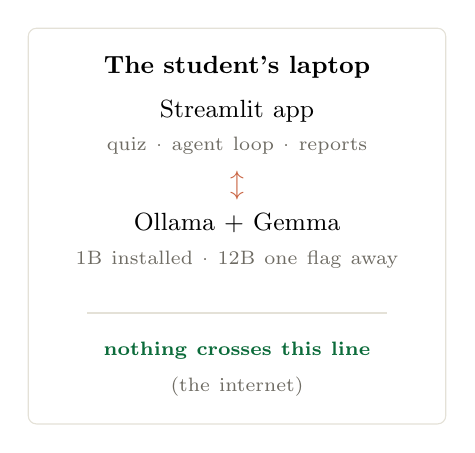
\begin{tikzpicture}
        \node[draw=line, fill=card, rounded corners=3pt, inner sep=10pt, text width=4.6cm, align=center] {
          {\small\bfseries The student's laptop}\\[4pt]
          {\small Streamlit app}\\
          {\scriptsize\color{muted}quiz · agent loop · reports}\\[3pt]
          {\color{clay}$\updownarrow$}\\[2pt]
          {\small Ollama + Gemma}\\
          {\scriptsize\color{muted}1B installed · 12B one flag away}\\[6pt]
          {\color{line}\rule{3.8cm}{0.6pt}}\\[3pt]
          {\scriptsize\color{okg}\bfseries nothing crosses this line}\\[1pt]
          {\scriptsize\color{muted}(the internet)}
        };
      \end{tikzpicture}
    \end{column}
  \end{columns}
\end{frame}

% ---------------------------------------------------------------- 10 DEMO
\begin{frame}{The 90-second live demo}
  \begin{enumerate}\setlength\itemsep{0.55em}
    \item {\small \textbf{Quiz} --- five questions, we miss the fraction item with the classic straight-across error.}
    \item {\small \textbf{Results} --- the agent finds the pattern, names the trick, builds the study guide.}
    \item {\small \textbf{``Practice until I've mastered it''} --- lesson appears; we answer wrong \emph{and type our flawed reasoning}.}
    \item {\small \textbf{The moment}: the agent reads our words, \textbf{switches teaching strategy, and explains why} --- attempt counter, approach, and streak all visible.}
    \item {\small We answer two fresh questions correctly $\rightarrow$ \textbf{Mastery demonstrated}, with a recap of which approaches it took.}
    \item {\small (And if we kept failing: a teacher hand-off report --- the agent knows its limits.)}
  \end{enumerate}
  \vspace{0.4em}
  \mutedtext{\small Everything shown runs live on this laptop. Wi-Fi can be off.}
\end{frame}

% ---------------------------------------------------------------- 11 ROADMAP
\begin{frame}{What's next \hfill {\normalsize\color{muted}same architecture, deeper Gemma}}
  \begin{itemize}\setlength\itemsep{0.7em}
    \item \textbf{Photograph your written work} --- Gemma 12B reads handwriting on-device; it transcribes, the verified bank judges. \mutedtext{\small (vision is in the model we already ship --- still zero cloud)}
    \item \textbf{Local tool use} --- Gemma emits structured tool calls; a local SymPy verifier proves every check deterministically. \mutedtext{\small (tool use for a model that doesn't natively support it --- via constrained JSON)}
    \item \textbf{Game mode} --- a three.js world where students move station to station; same agent brain underneath.
  \end{itemize}
  \vspace{0.7em}
  {\color{line}\hrule height 1pt}
  \vspace{0.5em}
  \kicker{How we score ourselves on the rubric}
  {\small
  \begin{tabular}{@{}llll@{}}
    \textbf{Gemma Integration 30\%} & \textbf{Innovation 30\%} & \textbf{Functionality 20\%} & \textbf{Writeup 20\%} \\
    \mutedtext{\scriptsize 4 roles, all guardrailed} & \mutedtext{\scriptsize goal-seeking tutor agent} & \mutedtext{\scriptsize live, tested, terminates} & \mutedtext{\scriptsize honest engineering story} \\
  \end{tabular}}
\end{frame}

% ---------------------------------------------------------------- 12 CLOSE
\begin{frame}
  \begin{center}
    \vspace{1.5em}
    {\rmfamily\fontsize{26}{32}\selectfont Build something people will remember ---\\ not because it's AI, but because it's genuinely useful.\par}
    \vspace{1.4em}
    {\small A student walks in confused about fractions.\\ Twenty minutes later they've \emph{proven} they understand --- and nothing about them ever left their laptop.}\par
    \vspace{1.6em}
    {\small\color{muted} github.com/EdTechDL/gemma-without-borders \,·\, live demo + clonable notebook}\par
    \vspace{0.6em}
    {\small Gokulakrishnan \,·\, Padmanabha \,·\, Taha \,·\, Naimah \,·\, Amarah}
  \end{center}
\end{frame}

\end{document}
